\documentclass[aspectratio=169,
				xcolor=table]{beamer}
				
% Load general definitions
\usepackage[utf8]{inputenc}
%\usepackage[T1]{fontenc}
\usepackage[brazil]{babel}
\usepackage{amsmath}
\usepackage{amsfonts}
\usepackage{amssymb}
\usepackage{graphicx}
\usepackage{verbatim}
\usepackage{cancel}
\usepackage{askmaps}
\usepackage{tabularx}
\usepackage[table]{xcolor}
%\usepackage{tikz}
\usepackage{multirow}
\usepackage{mathtools}
\usepackage{color, colortbl}
\usepackage{etoolbox}
\usepackage{pbox}
\usepackage{changepage}
\usepackage{xpatch}
\usepackage{array}
\usepackage{marvosym}
\usepackage{tabu}
\usepackage{multicol}
\usepackage{listings}
\usepackage{underscore}
\usepackage{filecontents}
\usepackage[]{algorithm2e}
\usepackage{ragged2e}

\newcolumntype{P}[1]{>{\centering\arraybackslash}m{#1}}
\definecolor{Gray}{gray}{0.75}
\definecolor{Gray2}{gray}{0.85}

\definecolor{lightBlue}{HTML}{DAE8FC}
\definecolor{Blue}{RGB}{51, 51, 204}

%\useinnertheme[lily]{rounded}
\usetheme{UniEvangelica}
%\usetheme{Copenhagen}
%\usetheme{Berlin}
%\usecolortheme{dolphin}
\tolerance=1
\emergencystretch=\maxdimen
\hyphenpenalty=10000
\hbadness=10000

\setbeamertemplate{navigation symbols}{}%remove navigation symbols


\let\olditem=\item% 
\renewcommand{\item}{\olditem \justifying}%
\def\center{\trivlist \centering\item\relax}
\def\endcenter{\endtrivlist}

\setbeamertemplate{itemize/enumerate body begin}{\large}
\setbeamertemplate{itemize/enumerate subbody begin}{\large}

\setbeamertemplate{itemize item}{\raisebox{0.1ex}{$\blacktriangleright$}\hskip0.1em}
\setbeamertemplate{itemize subitem}{\raisebox{0.1ex}{$\blacktriangleright$}\hskip0.1em}

\newcommand{\greenarrow}{\textcolor{green}{\rotatebox[origin=c]{180}{\MVArrowDown}}}

\newcommand{\redarrow}{\textcolor{red}{\MVArrowDown}}

%\newcommand{\ftable}{
%	\begin{table}
%		\large
%		\centering
%		\rowcolors{1}{\ifnumless{\rownum}{2}{Blue}{lightBlue}}{}
%}

\newenvironment{eftable}{
	\begin{table}
		\large
		\centering
		\rowcolors{1}{}{Blue}
		\rowcolors{1}{\ifnumless{\rownum}{2}{Blue}{lightBlue}}{}
	}
	{
	\end{table}
}


%\setbeamertemplate{frametitle}
%{
%	%\vspace*{-2em}	
%	\insertframetitle
%
%	 %\textcolor{white}{\LARGE \insertframetitle}
%
%}

% Specific definitions
\institute[]{\uppercase{Engenharia de Software}}
\title[]{Arquitetura e Organização de Computadores}
\subtitle[]{\uppercase{Memória Principal}}
\author[]{Prof. Alexandre Tannus}
\date{}

\AtBeginSection{\frame{\tableofcontents[currentsection]}}

\begin{document}

	\begin{frame}
		\titlepage
	\end{frame}

	\begin{frame}{Objetivos}
		\begin{itemize}
			\item Recordar a hierarquia de memórias
			\vspace{1em}
			\item Diferenciar memórias quanto às suas características
			\vspace{1em} 
			\item Contrastar os métodos de acesso à memória			
		\end{itemize}
	\end{frame}

	\begin{frame}
		\tableofcontents		
	\end{frame}	
	
	\section{Introdução}
	
	\begin{frame}{Introdução}
		\begin{itemize}
			\item Dispositivo responsável pelo armazenamento de informações
			\vspace{1em}
			\item Unidade básica de memória
			\begin{itemize}
				\item bit
			\end{itemize}
		\end{itemize}
	\end{frame}
	
	\begin{frame}{Hierarquia de memória}
		\begin{figure}[hbtp]
			\centering
			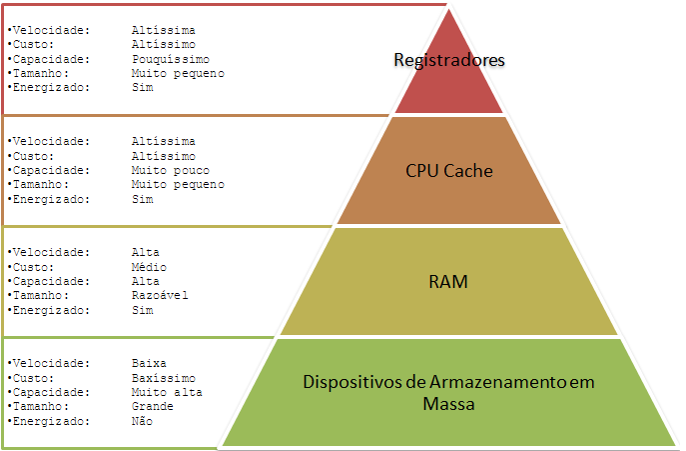
\includegraphics[height=0.83\textheight, keepaspectratio]{../figs/cap07/memoria.png}
		\end{figure}
	\end{frame}
		
	\begin{frame}{Tecnologias de memória}
		\begin{columns}
			\begin{column}{0.5\textwidth}
				\begin{itemize}
					\item Semicondutores 
					\begin{itemize}
						\item Memória RAM
						\item SSD
					\end{itemize}
					\vspace{1em}
					\item Magnética
					\begin{itemize}
						\item HD, disquete
					\end{itemize}
					\vspace{1em}
					\item Ótica
					\begin{itemize}
						\item CD, DVD
					\end{itemize}
				\end{itemize}
			\end{column}
			\begin{column}{0.5\textwidth}
				\begin{figure}[hbtp]
				\centering
				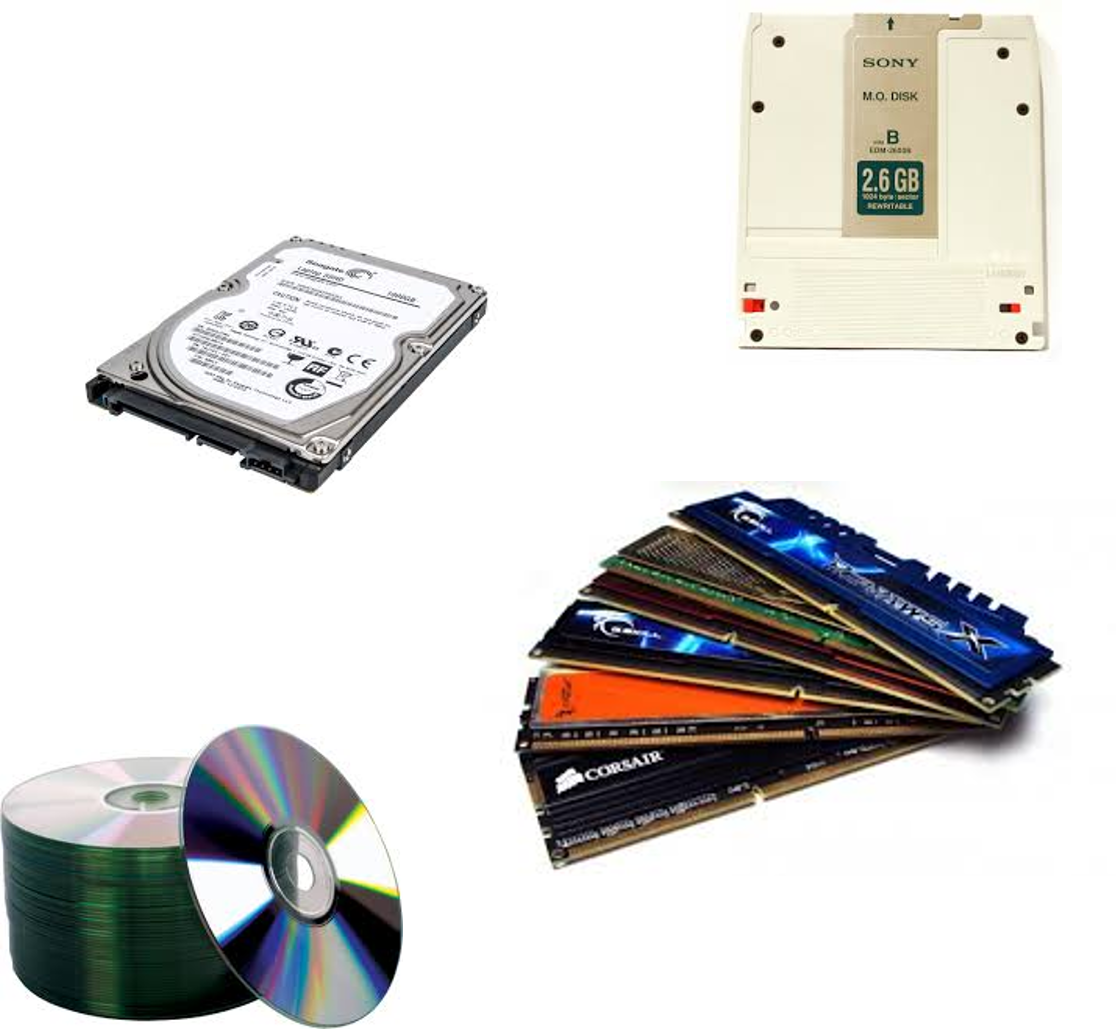
\includegraphics[height=.7\textheight, keepaspectratio]{../figs/cap07/tecnologias.png}
				\end{figure}
				
			\end{column}
		\end{columns}
	\end{frame}
	
	\begin{frame}{Tipo de armazenamento}
		\begin{itemize}
			\item Volátil
			\begin{itemize}
				\item Informação é apagada quando ocorre desenergização
				\item Exemplo: RAM
			\end{itemize}
			\vspace{1em}
			\item Não volátil
			\begin{itemize}
				\item Informação não é perdida com ausência de energia elétrica
				\item Exemplo: ROM	\end{itemize}
		\end{itemize}
	\end{frame}	
	
	\begin{frame}{Restrições de projeto}
		\begin{itemize}
			\item Capacidade da memória
			\vspace{1em}
			\item Custo por bit
			\vspace{1em}
			\item Velocidade de acesso
		\end{itemize}
	\end{frame}
	
	\begin{frame}{Célula de memória}
		\begin{itemize}
			\item Locais onde são armazenados os dados
			\vspace{1em}
			\item Referenciadas através do \textbf{endereço}
			\vspace{1em}
			\item Todas as células de uma memória possuem o mesmo número de bits

		\end{itemize}
	\end{frame}
	
	\begin{frame}{Endereçando memórias}
		\begin{figure}[hbtp]
			\centering
			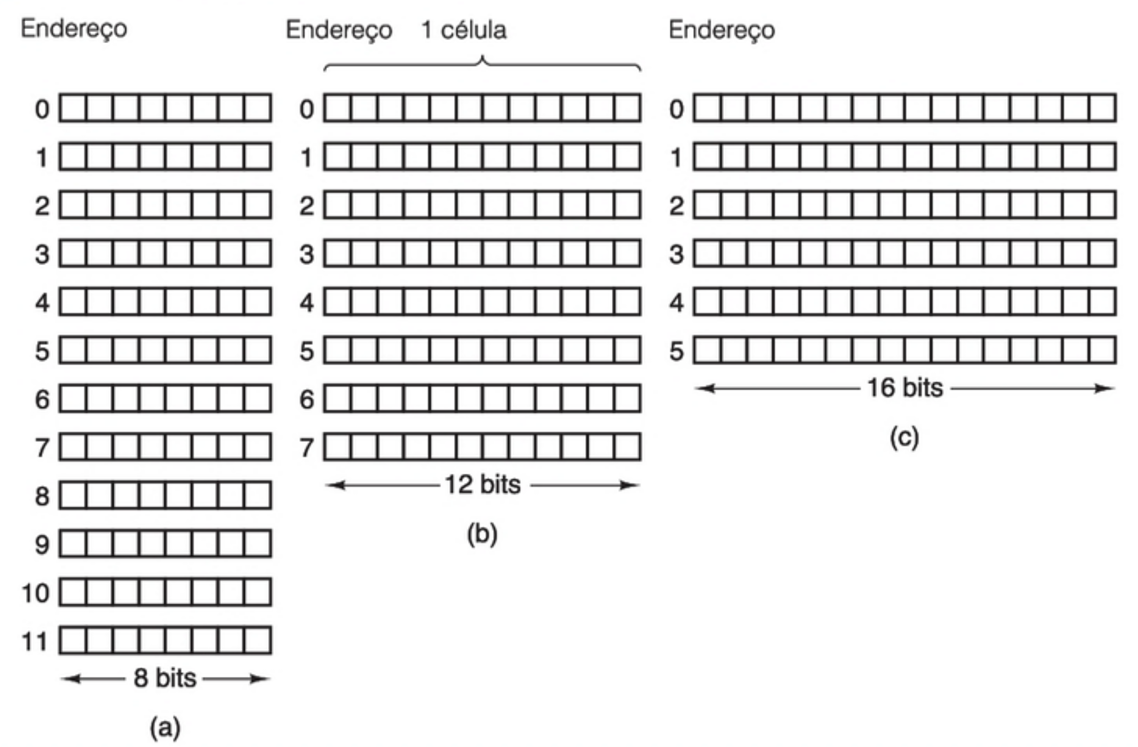
\includegraphics[height=0.8\textheight, keepaspectratio]{../figs/cap07/endercamento.png}
		\end{figure}
			
	\end{frame}
	
	\begin{frame}{Capacidade da memória}
		\begin{itemize}
			\item Quantidade de bits que a memória pode armazenar
			\vspace{1em}
			\item Depende de dois fatores
			\begin{itemize} 
				\item Tamanho da palavra
				\item Quantidade de palavras 
			\end{itemize}
		\end{itemize}
	\end{frame}

	\begin{frame}{Princípio da localidade}
		\begin{itemize}
			\item Localidade espacial
			\begin{itemize}
				\item Quando um determinado item é referenciado, itens com endereços de memória próximo a ele tendem a ser logo referenciados
			\end{itemize}
			\vspace{1em}
			\item Localidade temporal
			\begin{itemize}
				\item Quando um determinado item é referenciado, a tendência é que ele seja novamente referenciado dentro de um curto período de tempo
			\end{itemize}
		\end{itemize}
		
	\end{frame}		
	
	\section{Métodos de Acesso}
	\begin{frame}{Métodos de acesso}
		\begin{itemize}
			\item Sequencial
			\vspace{1em}
			\item Direto
			\vspace{1em}
			\item Aleatório
			\vspace{1em}
			\item Associativo
		\end{itemize}
	\end{frame}
	
	\begin{frame}{Acesso Sequencial}
		\begin{itemize}
			\item Dados organizados de forma sequencial
			\vspace{1em}
			\item Exemplo: fitas magnéticas
					\begin{figure}[hbtp]
			\centering
			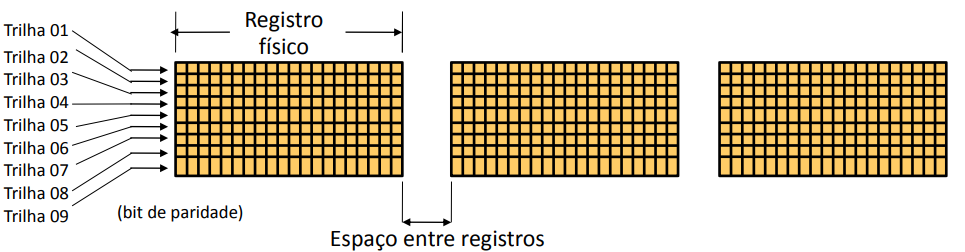
\includegraphics[height=0.4\textheight, keepaspectratio]{../figs/cap07/acessodireto}
		\end{figure}
		\end{itemize}
	\end{frame}
	
	\begin{frame}{Acesso Direto}
		\begin{itemize}
			\item Cada bloco de dados possui um endereço único, baseado na localização física
			\vspace{1em}
			\item O acesso é feito através do acesso direto a uma vizinhança genérica do registro, e em seguida por uma busca sequencial 
			\vspace{1em}
			\item O tempo de acesso é variável
		\end{itemize}
	\end{frame}
	
	\begin{frame}{Acesso aleatório}
		\begin{itemize}
			\item Cada posição de memória possui um endereço único
			\vspace{1em}
			\item O tempo de acesso a uma posição é constante, sendo independente dos acessos anteriores
		\end{itemize}
	\end{frame}
	
	\begin{frame}{Acesso associativo}
		\begin{itemize}
			\item Tipo de acesso aleatório que compara simultaneamente certo número de bits de uma palavra com todas as
palavras da memória, determinando quais delas contém o mesmo padrão de bits
			\vspace{1em}
			\item Uma palavra é buscada com base em parte de seu conteúdo, e não de acordo com o seu endereço
		\end{itemize}
	\end{frame}
	
	\begin{frame}{Parâmetros de desempenho}
		\begin{itemize}
			\item Tempo de acesso (latência)
			\begin{itemize}
				\item Memórias de \alert{acesso aleatório} - tempo gasto para uma operação de leitura ou escrita
				\item Memórias de acesso \alert{não aleatório} - tempo gasto para posicionar o mecanismo de leitura-escrita no local desejado
			\end{itemize}
			\vspace{1em}
			\item Tempo de ciclo
			\begin{itemize}
				\item Tempo para que a memória esteja novamente disponível para acesso
				\item Referente ao barramento do sistema
			\end{itemize}
			\vspace{1em}
			\item Taxa de transferência
			\begin{itemize}
				\item Taxa que os dados podem ser transferidos de e para uma memória
			\end{itemize}
		\end{itemize}
	\end{frame}
	
	\begin{frame}{Taxa de transferência - Cálculo}
		\begin{itemize}
			\item Memórias de acesso aleatório
			\begin{itemize}
				\item $\frac{1}{tempo \enspace de \enspace ciclo}$
			\end{itemize}
			\vspace{1em}
			\item Memórias de acesso não aleatório
			\begin{itemize}
				\item $T_N = T_A +\frac{n}{R}$
				\begin{itemize}
				\item $T_N$ - tempo médio para leitura ou escrita de \textit{n} bits
				\item $T_A$ - tempo de acesso médio
				\item $n$ - número de bits
				\item $R$ - taxa de transferência em bits por segundo				
				\end{itemize}
			\end{itemize}
		\end{itemize}
	\end{frame}		
	
	\section{Memória de Acesso Aleatório - RAM}
	\begin{frame}{Memória Principal}
		\begin{itemize}
			\item Armazenamento massivo de informações
			\begin{itemize}
				\item Atualmente na faixa de gigabytes
			\end{itemize}
			\vspace{1em}
			\item Memórias de acesso aleatório
			\begin{itemize}
				\item RAM (\textit{Random Access Memory})
				\item ROM (\textit{Read Only Memory})

			\end{itemize}
		\end{itemize}
	\end{frame}
	
	\begin{frame}{Tipos de memória}
		\begin{figure}[hbtp]
			\centering
			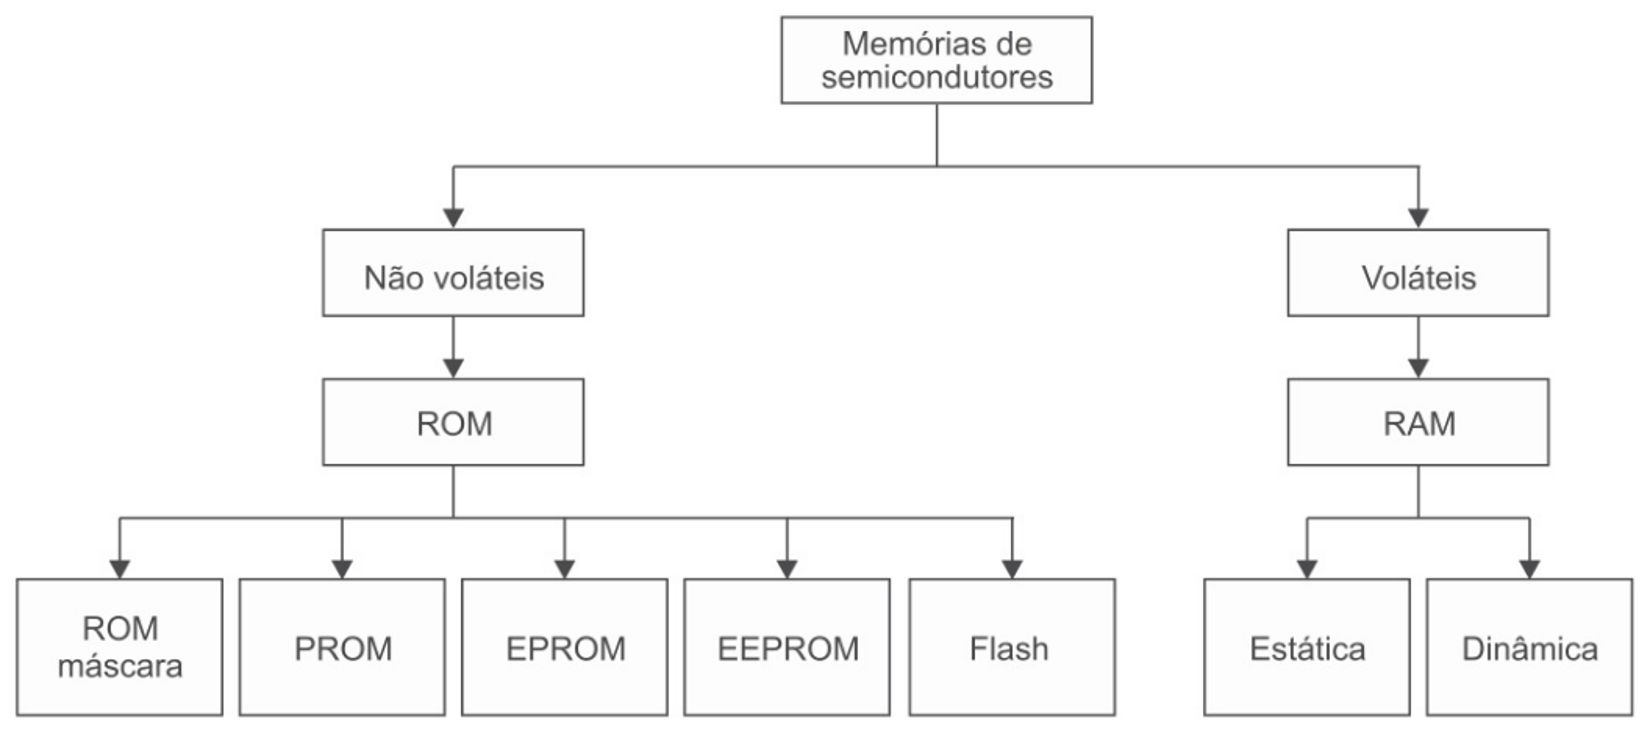
\includegraphics[width=0.9\textwidth, keepaspectratio]{../figs/cap07/semicond.png}
		\end{figure}
	\end{frame}
	
	\begin{frame}{Memória RAM}		
		\begin{itemize}
			\item Memória volátil de acesso aleatório
			\vspace{1em}
			\item Leitura e escrita
			\vspace{1em}
			\item Tipos
			\begin{itemize}
				\item \textbf{Estática (SRAM – \textit{Static} RAM)}
				\item \textbf{Dinâmica (DRAM – \textit{Dynamic} RAM)}
				\item Vídeo (VRAM - \textit{Video} RAM)
				\item WRAM (\textit{Window} RAM) 
				\item CMOS RAM
			\end{itemize}
		\end{itemize}		
	\end{frame}
	
	\subsection{RAM Dinâmica}
	\begin{frame}{RAM Dinâmica}
		\begin{itemize}
			\item Local onde são armazenados os programas
			\vspace{1em}
			\item Necessidade de \textit{refresh} para manter dados
		\end{itemize}
	\end{frame}
	
	\begin{frame}{Características DRAM}
		\begin{itemize}
			\item Baixo custo
			\vspace{1em}
			\item Baixo consumo de energia
			\vspace{1em}
			\item Alto poder de integração
			\begin{itemize}
				\item Maior capacidade de armazenamento
			\end{itemize}
			\vspace{1em}
			\item Lenta
		\end{itemize}
	\end{frame}
	
	\begin{frame}{\textit{\textit{Synchronous} DRAM (SDRAM)}}
		\begin{itemize}
			\item \textit{Clock} interno para leitura e gravação
			\vspace{1em}
			\item Maior velocidade de acesso
			\begin{itemize}
				\item \textit{Double Data Rate} (DDR)
			\end{itemize}

		\end{itemize}
	\end{frame}
	
	\begin{frame}{Memórias DDR}
		\begin{eftable}  
			\resizebox{\textwidth}{!}{%
			\begin{tabular}{cccccc}
				{\color[HTML]{FFFFFF} Tipo} & {\color[HTML]{FFFFFF} \begin{tabular}[c]{@{}c@{}}Ano de \\ Lançamento\end{tabular}} & {\color[HTML]{FFFFFF} \begin{tabular}[c]{@{}c@{}}Quantidade de \\ pinos (DIMM)\end{tabular}} & {\color[HTML]{FFFFFF} \begin{tabular}[c]{@{}c@{}}Clock do \\ Barramento (MHz)\end{tabular}} & {\color[HTML]{FFFFFF} \begin{tabular}[c]{@{}c@{}}Taxa de \\ Transferência\end{tabular}} & {\color[HTML]{FFFFFF} \begin{tabular}[c]{@{}c@{}}Tensão de \\ Operação (V)\end{tabular}} \\
				DDR                         & 2000                                                                                & 184                                                                                          & 100 - 200                                                                                   & 200 - 400                                                                               & 2,5                                                                                      \\
				DDR2                        & 2003                                                                                & 240                                                                                          & 100 - 266                                                                                   & 400 - 1066                                                                              & 1,8                                                                                      \\
				DDR3                        & 2007                                                                                & 240                                                                                          & 100 - 266                                                                                   & 800 - 2133                                                                              & 1,5                                                                                      \\
				DDR4                        & 2014                                                                                & 288                                                                                          & 133 - 267                                                                                   & 2133 - 4266                                                                             & 1,2                                                                                     
			\end{tabular}
			}
		\end{eftable}
	\end{frame}
	
	\begin{frame}{Memórias DDR}
		\begin{figure}[hbtp]
		\centering
		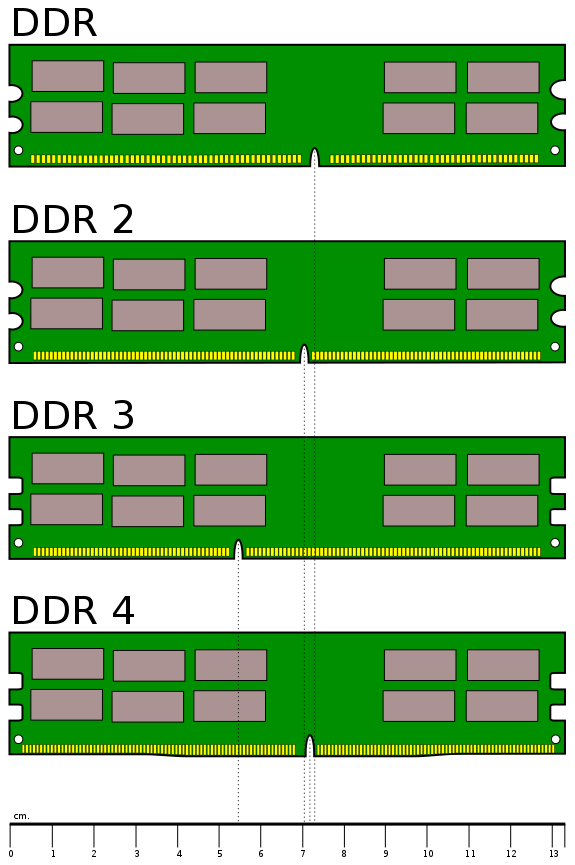
\includegraphics[height=0.8\textheight, keepaspectratio]{../figs/cap07/ddr.png}
		\end{figure}
		
	\end{frame}
	
	\subsection{RAM Estática}
	\begin{frame}{\textit{Static RAM} - SRAM}
		\begin{itemize}
			\item Construídas a partir de \textit{flip-flops}
			\vspace{1em}
			\item Voláteis
			\vspace{1em}
			\item Não necessitam de \textit{refresh}
			\vspace{1em}
			\item Principal uso
			\begin{itemize}
				\item Memória Cache
			\end{itemize}			
		\end{itemize}	
	\end{frame}
	
	\begin{frame}{Tecnologias de Construção}
		\begin{itemize}
			\item Bipolar
			\vspace{1em}
			\item CMOS
			\vspace{1em}
			\item NMOS
		\end{itemize}
	\end{frame}	

	\begin{frame}{Célula SRAM básica}
		\begin{figure}[hbtp]
		\centering
		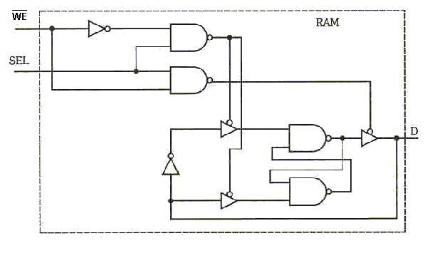
\includegraphics[height=0.8\textheight, keepaspectratio]{../figs/cap07/celulaSRAM}
		\end{figure}
		
	\end{frame}

	\begin{frame}{Célula SRAM básica}
		\begin{figure}[hbtp]
		\centering
		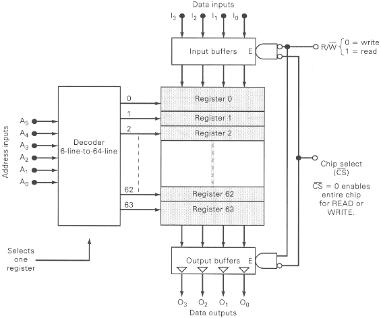
\includegraphics[height=0.8\textheight, keepaspectratio]{../figs/cap07/sram64x4}
		\end{figure}
		
	\end{frame}
	
%	\begin{frame}
%		É um exemplo de memória SRAM:
%		\begin{enumerate}[a]
%			\item DDR.
%			\item flash.
%			\item DDR2.
%			\item cache.
%			\item disco rígido.
%		\end{enumerate}
%	\end{frame}	
	
	\begin{frame}{DRAM x SRAM}
		\begin{eftable}
%			\resizebox{\textwidth}{!}{%
			\begin{tabular}{l|c|c}
				{\color[HTML]{FFFFFF} Característica}                                & {\color[HTML]{FFFFFF} \begin{tabular}[c]{@{}c@{}}RAM Dinâmica \\ (DRAM)\end{tabular}} & {\color[HTML]{FFFFFF} \begin{tabular}[c]{@{}c@{}}RAM Estática \\ (SRAM)\end{tabular}} \\
				\begin{tabular}[c]{@{}l@{}}Circuito de \\ armazenamento\end{tabular} & Capacitor                                                                             & Flip-flop                                                                             \\
				\begin{tabular}[c]{@{}l@{}}Taxa de \\ transferência\end{tabular}     & \begin{tabular}[c]{@{}l@{}}Menor do que a \\ do processador\end{tabular}              & \begin{tabular}[c]{@{}l@{}}A mesma do \\ processador\end{tabular}                     \\
				Latência                                                             & Alta                                                                                  & Baixa                                                                                 \\
				Densidade                                                            & Alta                                                                                  & Baixa                                                                                 \\
				\begin{tabular}[c]{@{}l@{}}Consumo de \\ energia\end{tabular}        & Baixo                                                                                 & Alto                                                                                  \\
				Custo   & Baixo & Alto                                                  
			\end{tabular}
%			}
		\end{eftable}
	\end{frame}
	
	\section{Read Only Memory - ROM}
	\begin{frame}{\textit{Read Only Memory} (ROM)}
		\begin{itemize}
			\item Memória não volátil somente de leitura
			\vspace{1em}
			\item Utilização
			\begin{itemize}
				\item BIOS (\textit{Basic Input/Output System})
				\item Bibliotecas de uso frequente
				\item Programas do sistema
				\item Tabelas de função
			\end{itemize}
		\end{itemize}
	\end{frame}	
	
	\begin{frame}{Tipos de ROM}		
		\begin{eftable}
			\centering
			\begin{tabular}{c|c|c}
				{\color[HTML]{FFFFFF} Tipo}                                             & {\color[HTML]{FFFFFF} Apagamento} & {\color[HTML]{FFFFFF} Mecanismo de escrita} \\
				ROM (\textit{Read Only Memory}) & Impossível & Máscaras \\
				PROM (\textit{Programmable} ROM)  & Impossível & Eletricamente \\
				EPROM (\textit{Erasable} PROM)       & Luz ultravioleta & Eletricamente \\
				EEPROM (Electrically   EPROM) & Eletricamente & Eletricamente\\
				Flash & Eletricamente & Eletricamente
			\end{tabular}
		\end{eftable}		
	\end{frame}
		
	\section{Exercícios}
	% Introdução
		%Hierarquia de memórias
	\begin{frame}{Questão 01 - TRE-BA 2016}
		No que se refere à hierarquia de memória tradicional, assinale a opção que relaciona os tipos de memória em ordem crescente do parâmetro velocidade de acesso.
		\vspace{1em}
		\begin{enumerate}[a]
		\large
			\item memória cache, registradores, memória principal, memória secundária
			\item memória principal, memória secundária, memória cache, registradores
			\item memória secundária, memória principal, memória cache, registradores
			\item registradores, memória principal, memória secundária, memória cache
			\item memória principal, registradores, memória secundária, memória cache		
		\end{enumerate}
	\end{frame}
	
	\begin{frame}{Questão 02 - SP-URBANISMO 2014}
		No contexto de arquitetura de computadores, os discos rígidos e as memórias do tipo RAM são exemplos, respectivamente, na hierarquia de memória de um computador, de componentes denominados
		\begin{enumerate}[a]
			\item memória primária e memória secundária
			\item memória primária e memória terciária
			\item memória secundária e memória primária.
			\item memória terciária e memória primária.
			\item memória terciária e memória secundária
		\end{enumerate}
	\end{frame}
	
	\begin{frame}{Questão 03 - IF-PA 2016}
		Para se obter um bom compromisso entre desempenho e custo, um computador emprega memórias de diversos tipos de tecnologias. Dentre Cache, Memória Principal e Registradores, as memórias que possuem maior capacidade de armazenamento e maior velocidade de acesso são, respectivamente:
		\begin{enumerate}[a]
			\item Cache e Registradores.
			\item Memória Principal e Registradores.
			\item Memória Principal e Cache.
			\item Registradores e Cache.
			\item Cache e Memória Principal.
		\end{enumerate}
	\end{frame}

		%Endereçamento de memória
	\begin{frame}{Questão 04 - CRF-PI 2016}
		Quanto a organização da memória, a quantidade de bits em um endereço está relacionada a:
		\begin{enumerate}[a]
			\item Quantidade média de células endereçáveis.
			\item Mínima quantidade de células endereçáveis. 
			\item Máxima quantidade de células endereçáveis
			\item Mínima quantidade de células endereçadas.			
		\end{enumerate}
	\end{frame}
	
	\begin{frame}{Questão 05 - UNIRIO 2016}
		Uma determinada memória RAM é fabricada com capacidade para armazenar 512 Mbits. Sabe-se que cada posição endereçável da memória armazena 32 bits.
		
		Qual é o número mínimo de bits a ser utilizado para que se possa endereçar toda essa memória? 
		\begin{enumerate}[a]
			\item 8
			\item 16
			\item 24
			\item 32
			\item 48
		\end{enumerate}
	\end{frame}
	
	\begin{frame}{Questão 06 - PC-AC 2015}
		Considere um sistema computacional que possui instalados 4GB de memória principal. Sabendo-se que sua célula de memória apresenta 64 bits (o mesmo tamanho da palavra), o tamanho mínimo de barramento de endereços desse sistema é:
		\begin{enumerate}[a]
			\item 26
			\item 30
			\item 35
			\item 29
			\item 42
		\end{enumerate}
	\end{frame}

	\begin{frame}{Questão - Transpetro 2011}		
		\begin{columns}
			\begin{column}{0.65\textwidth}
				Segue-se o trecho final de uma memória principal, onde o endereço FFF representa a maior posição endereçável. Todos os números são apresentados em hexadecimal.
	
				O número máximo de células que essa memória pode conter será igual a
				\begin{enumerate}[a]
					\item	512
					\item	1024
					\item	2048
					\item	4096
					\item	8192			
				\end{enumerate}			
			\end{column}
			\begin{column}{0.35\textwidth}
				\begin{figure}
					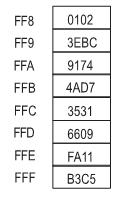
\includegraphics[height=0.7\textheight, keepaspectratio]{../figs/cap07/memquestion.png}
				\end{figure}			
			\end{column}
		\end{columns}		
	\end{frame}	
	
		%Métodos de acesso
	\begin{frame}{Questão 07 - POSCOMP 2014}
		Sobre os métodos de acesso das unidades de dados, considere as afirmativas a seguir.
		\begin{enumerate}[I]
			\large
			\item No acesso sequencial, a informação de endereçamento armazenada é usada para separar registros e auxiliar no processo de recuperação.
			\item No acesso direto, os blocos têm um endereçamento exclusivo, baseado no local físico.
			\item No acesso aleatório, o tempo para acessar um determinado local é constante.
			\item No acesso associativo, uma palavra é recuperada com base em uma parte do seu endereço.
		\end{enumerate}
	\end{frame}	
	
		% Memória RAM
	\begin{frame}{Questão 08 - COBRA Tecnologia S/A 2015}
		Quanto à memória RAM, qual das alternativas faz uma afirmação verdadeira?
		\begin{enumerate}[a]
			\item É uma memória de baixo desempenho, em relação ao HardDisk.
			\item É um tipo de memória volátil.
			\item Pode-se expandir com o uso de CD-ROM.
			\item Seu método de gravação se dá por meio magnético.
			\item Possui trilhas e setores para delimitar as regiões de dados.
		\end{enumerate}
	\end{frame}	
	
	\begin{frame}{Questão 09 - HOB 2015}
	
		A memória RAM possui como características, EXCETO:
		
		\begin{enumerate}[a]
			\large
			\item Armazena os dados que o processador utiliza para trabalhar.
			\item É uma memória não volátil, pois armazena seus dados temporariamente.
			\item SRAM e DRAM são tipos de tecnologia de memória RAM muito utilizados.
			\item A quantidade de memória influencia diretamente na capacidade de trabalho do computador.
		\end{enumerate}

	\end{frame}	
	
	\begin{frame}{Questão 10 - SESAU-RO 2017} 
		Considere as seguintes assertivas acerca de arquitetura de computadores e tipos de memórias:
		\begin{enumerate}[I]
			\item A memória cache é uma memória do tipo não volátil utilizada para armazenamento seguro de dados em longo prazo.
			\item Os registradores são dispositivos de armazenamento temporário (volátil), localizados no interior do processador (CPU).
			\item Duas características das memórias ROM é que elas são do tipo volátil e não podem ser acessadas de modo aleatório, apenas sequencial.
		\end{enumerate}
	\end{frame}

	\begin{frame}{Questão 11 - CRF-SC 2012}
		Identifique as características da memória RAM dinâmica (DRAM). 
		
		\begin{enumerate}[I]
			\large
			\item Difícil integração (pouca capacidade em muito espaço). 
			\item Baixo consumo. 
			\item Alto consumo. 
			\item Rápida. 
			\item Lenta, pois necessita de refresh. 
		\end{enumerate}
	\end{frame}

%	\begin{frame}{Questão 12 - MEC 2015}
%		Um computador com memória principal capaz de armazenar palavras de 16 bits em cada uma de suas N células e com barramento de endereço que tenha 14 bits de tamanho terá uma capacidade total de armazenamento da memória principal de 8.192 bytes.
%	\end{frame}

		%Memória ROM
	\begin{frame}{Questão 12 - TRF - 1${}^a$ REGIÃO 2014}
		Parte da memória principal de um computador, a ROM é uma memória apenas de ......, que armazena os dados ...... . Contém programas que não podem ser ...... pelo usuário.

		Os termos que preenchem corretamente as lacunas do texto são: 
			\begin{enumerate}[a]
				\item	acesso imediato, em arquivos, gravados. 
				\item	gravação, no disco rígido, decodificados. 
				\item	acesso secundário, temporariamente, acessados. 
				\item	programação, do sistema operacional, alterados.
				\item	leitura, de modo permanente, apagados.	
			\end{enumerate}
	\end{frame}
	
	\begin{frame}{Questão 13 - UFGD 2014}
		Em um computador existe memórias voláteis (que necessita de energia para armazenar dados) e não voláteis (que não necessitam de energia para armazenar). Qual das alternativas a seguir apresenta APENAS memórias não-voláteis?
		
		\begin{enumerate}[a]
			\item	RAM, DRAM, Cache.
			\item	Flash, SRAM, ROM.
			\item	PROM, EPROM, EEPROM
			\item	Cache, Flash, DRAM.
			\item	DRAM, ROM, EPROM.		
		\end{enumerate}
	\end{frame}
	
	\begin{frame}{Questão 14 - UFF 2017}
		Para que um programa BIOS seja atualizado, ele deve ser gravado em memórias do tipo: 
		\begin{enumerate}[a]
			\item RAM ou ROM.
			\item EEPROM ou cache. 
			\item Flash ou ROM.
			\item Flash ou EEPROM.
			\item  EEPROM ou RAM. 			
		\end{enumerate}
	\end{frame}
	
	\begin{frame}{Referências}
		\nocite{Englander2011}
		\nocite{Paixao2014}
		\nocite{Stallings2010}
    	\bibliographystyle{plain}
    	\bibliography{../refs} 			
	\end{frame}	
	
	\begin{frame}{}
	\end{frame}
	
\end{document}
